\documentclass[solution, letterpaper]{cs20inclass}
\usepackage{enumerate}
\usepackage{tikz}
\usepackage{pgf}
\usepackage{tikz}
\usepackage{hyperref}
\usepackage{ dsfont }
\usepackage{amsmath}
\begin{document}
\header{15}{Wednesday, March 02, 2016}

\noindent Author: Crystal Chang

\paragraph*{Executive Summary}
\begin{enumerate}
\item \textbf{Definition of Recursive Data Types:} common way of defining mathematical objects, which says how to construct new data elements from previous ones.
\begin{itemize}
\item {\em Base Case(s):} specify that some known mathematical elements are in the data type
\item {\em Constructor Rule(s):} specify how to construct new data elements from previously constructed elements or from base elements.
\item {\em “Nothing else” (generally implicit):} the only way you can get whatever is you defining is by starting from the base case(s) and applying the constructor rule(s) one or more times.
\end{itemize}

\item \textbf{The Principle of Structural Induction:} to prove P(x) holds for all x in a recursively defined set S, prove
\begin{itemize}
\item {\em Basis Step:} P(b) is true for each base case element $b \in S$, and 
\item {\em Recursive Step:} P(c($x_1$,...,$x_k$)) for each constructor c, assuming as the induction hypothesis that P($x_1$),..., and P($x_k$) all hold.
\end{itemize}
\end{enumerate}

%% PROBLEM 1 %%
\problem Recursive Definition:
\subproblem There's an error in the following definition of the set of even integers (E). Find the error and fix it. 
\begin{itemize}
\item Base Case:  $0\in E$
\item Constructor Rule: For any element x in E, x+2 is in E. 
\item “Nothing else” (generally implicit): Nothing is in E unless it is obtained from the base case and constructor rule.
\end{itemize}
\subproblem Give a recursive definition of the natural numbers $\mathbb{N}$.
\subproblem Give a recursive definition of the sequence $b_n$, $b_n=2n+5,  n\in\mathbb{N}$
\pagebreak

\begin{solution}
\subsolution  It doesn't include negative Even Integer. There should be one more constructor rule “x-2 is in EI”.
\subsolution 
\begin{itemize}
\item Base Cases:  $1\in \mathbb{N}$
\item Constructor Rule: If $n\in\mathbb{N}$, then $n+1\in\mathbb{N}$.
\item “Nothing else” (generally implicit): Nothing is in $\mathbb{N}$ unless it is obtained from the base case and constructor rule.
\end{itemize}
\subsolution
\begin{itemize}
\item Base Cases:  $b_1=7$
\item Constructor Rule: $b_{n+1}=b_n+2$ for $n\in\mathbb{N}$
\item “Nothing else” (generally implicit): Nothing is in $b_n$ unless it is obtained from the base case and constructor rule.
\end{itemize}
\end{solution}

%% PROBLEM 2 %%
\problem Let S be the set defined as follows:
\begin{itemize}
\item Base Case: $(1,2) \in S$
\item Constructor Rules: If $(x,y)\in S$, then C1: $(x+2, y) \in S$ and C2: $(y,x) \in S$ 
\end{itemize}
\subproblem Is $(4,3)\in S$? If it is, how can you derive it from (1,2)?
\subproblem Use induction to prove that $(2n+2, 2n+1)\in S$ for all n $\in \mathbb{N}$.

\begin{solution}
\subsolution Yes, it is. Apply C1 to (1,2), we can get (3,2); Apply C2 to (3,2), we can get (2,3); Apply C1 to (2,3), we can get (4,3).
\subsolution Let P(n): $(2n+2, 2n+1)\in S$. We must show that for all $n\in\mathbb{N}, P(n)$.
\begin{itemize}
\item Base case: When n=1, $(4,3)\in S$. (Already proved in (A))
\item Induction step: \\
Assuming P(n): $(2n+2, 2n+1)\in S$ holds, we want to prove that $P(n+1): (2(n+1)+2, 2(n+1)+1)=(2n+4, 2n+3)\in S$.\\
Apply C1 to (2n+2, 2n+1), we then could get $(2n+4, 2n+1)\in S$. Then apply C2 to (2n+4, 2n+1), we could get $(2n+1, 2n+4)\in S$. Then, apply C1 to (2n+1, 2n+4), then we can get $(2n+3, 2n+4)\in S$. Finally, apply C2 again to (2n+3, 2n+4), then we can get $(2n+4, 2n+3)\in S$.
\end{itemize}
\end{solution}

%% PROBLEM 3%%
\problem (Bonus) The set of Pythagoras trees:\\
The shape of Pythagoras tree is built by recursively feeding the axiom through the production rules. Each character of the input string is checked against the rule list to determine which character or string to replace it with in the output string. In this example, a '1' in the input string becomes '11' in the output string, while '[' remains the same. 
\begin{itemize}
\item variables: 0,1
\item constants: [,]
\item axiom: 0
\item rules: $(1\rightarrow 11), (0\rightarrow 1[0]0)$
\end{itemize}
\subproblem Give a recursive definition of the  Pythagoras tree.
\subproblem List the first 4 elements.
\subproblem This string can be drawn as an image by using turtle graphics, where each symbol is assigned a graphical operation for the turtle to perform. For example, in the sample above, the turtle may be given the following instructions:
\begin{itemize}
\item 0: draw a line segment ending in a leaf
\item 1: draw a line segment
\item $[$: push position and angle, turn left 45 degrees
\item $]$: pop position and angle, turn right 45 degrees
\end{itemize}
Applying the graphical rules listed above to the earlier recursion, we could get the graphical representation of axiom, 1st and 2nd recursion as the following :\\
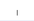
\includegraphics[width=2cm]{0} 
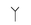
\includegraphics[width=2cm]{1}
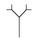
\includegraphics[width=2cm]{2}\\
Draw out the graphical representation of the 3rd and 4th recursion.

\begin{solution}
\subsolution
\begin{itemize}
\item Base Case:  $0\in E$
\item Constructor Rule:  $(1\rightarrow 11), (0\rightarrow 1[0]0)$
\item “Nothing else” (generally implicit): Nothing is in the set of Pythagoras tree unless it is obtained from the base case and constructor rule.
\end{itemize}
\subsolution 
\begin{itemize}
\item axiom:	0
\item 1st recursion:	$1[0]0$
\item 2nd recursion: $11[1[0]0]1[0]0$
\item 3rd recursion:	$1111[11[1[0]0]1[0]0]11[1[0]0]1[0]0$
\end{itemize}
\subsolution
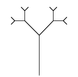
\includegraphics[width=2cm]{3} 
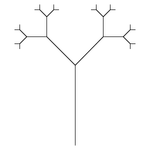
\includegraphics[width=2cm]{4}
\end{solution}


%% PROBLEM 4 %%
\problem (Bonus) Let S be the set defined as follows:
\begin{itemize}
\item Base Case: $(0,0) \in S$
\item Constructor Rules: If $(a,b)\in S$, then C1: $(a, b+1) \in S$, C2: $(a+1,b+1)\in S$ and C3: $(a+2, b+1)\in S$ 
\end{itemize}
\subproblem List 5 elements.
\subproblem Use structural induction to prove that for every $(a,b)\in S, a\leq 2b$.

\begin{solution}
\subsolution (0,1), (1,1), (2,1), (1,2), (2,2)...
\subsolution
\begin{itemize}
\item Basis step: By the base case of the definition of S, $(0,0)\in S$. $0\leq2(0)$.
\item Recursive step: \\
Now consider the constructor rule in the definition of S. Assume elements $a,b\in S$ and $ a\leq 2b$. We must  show that $a\leq2(b+1)$, $(a+1)\leq2(b+1)$ and $(a+2)\leq2(b+1)$.
\subitem 1. prove $a\leq2(b+1)$:  $a\leq2b\rightarrow a\leq(2b+2)=2(b+1)$
\subitem 2. prove $(a+1)\leq2(b+1)$: $a\leq2b \rightarrow (a+1)\leq(2b+1)\leq(2b+2)=2(b+1)$
\subitem 3. prove $(a+2)\leq2(b+1)$:  $a\leq2b \rightarrow (a+2)\leq(2b+2)=2(b+1)$
\end{itemize}
\end{solution}

\end{document}